\section{Results and Discussion}\label{sec:results}
All results come from 130 runs (10 per combination) measured on the platform described in Section~\ref{sec:case-study}; all values are means with 95\,\% confidence intervals unless stated otherwise. Table~\ref{tab:results} summarizes the results. The raw measurements and the scripts that produce every table and figure are in the repository of the project.

\begin{table}[H]
\caption{Results by condition and attack (mean $\pm$ 95\,\% CI, $n=10$ runs per row). Replies/issued is $A_{iss}$ and Replies/sched.\ is $A_{sch}$; Removed is the percentage of attack packets that do not reach the PLC network; PLC down is the number of runs in which the PLC runtime had stopped after the attack.}\label{tab:results}
\centering\scriptsize
\setlength{\tabcolsep}{3pt}
\begin{tabular}{llrrrrr}
\toprule
Attack & Scen. & Replies/ & Replies/ & RTT p95 & Removed & PLC\\
 & & issued (\%) & sched. (\%) & (ms) & (\%) & down\\
\midrule
None & E0 & 100.0 & 100.0 & 0.86 $\pm$ 0.01 & -- & 0/10\\
\midrule
TCP SYN & E1 & 99.2 $\pm$ 0.2 & 99.0 $\pm$ 0.3 & 260 $\pm$ 6 & 2.0 $\pm$ 0.4 & 0/10\\
 & E2 & 3.4 $\pm$ 0.9 & 0.7 $\pm$ 0.2 & 359 $\pm$ 94 & 68.8 $\pm$ 1.1 & 0/10\\
 & E3 & 75.8 $\pm$ 4.0 & 48.2 $\pm$ 9.3 & 310 $\pm$ 56 & 99.9 & 0/10\\
\midrule
UDP & E1 & 100.0 & 100.0 & 4.3 $\pm$ 0.5 & 0.0 & 0/10\\
 & E2 & 66.7 $\pm$ 16.8 & 50.4 $\pm$ 23.1 & 249 $\pm$ 109 & 54.2 $\pm$ 0.8 & 0/10\\
 & E3 & 73.3 $\pm$ 4.5 & 41.9 $\pm$ 8.2 & 346 $\pm$ 51 & 99.7 $\pm$ 0.1 & 0/10\\
\midrule
ICMP & E1 & 100.0 $\pm$ 0.1 & 100.0 $\pm$ 0.1 & 21.0 $\pm$ 1.0 & 2.2 $\pm$ 0.4 & 0/10\\
 & E2 & 49.1 $\pm$ 26.3 & 41.7 $\pm$ 27.8 & 203 $\pm$ 164 & 63.1 $\pm$ 2.1 & 0/10\\
 & E3 & 77.3 $\pm$ 5.3 & 48.7 $\pm$ 10.3 & 391 $\pm$ 22 & 100.0 & 0/10\\
\midrule
Modbus & E1 & 100.0 & 100.0 & 2.0 $\pm$ 1.3 & 0.0 & 10/10\\
 & E2 & 99.7 & 99.7 & 0.9 $\pm$ 0.8 & 0.0 & 10/10\\
 & E3 & 100.0 & 100.0 & 1.1 & 30.8 $\pm$ 3.2 & 6/10\\
\bottomrule
\end{tabular}

\end{table}

\subsection{Service Availability}
Figure~\ref{fig:avail} shows the availability of the SCADA client during the attack. The baseline E0 gives 100\,\% of valid replies and an RTT p95 of 0.86~ms. Without the IPS (E1), the SYN, UDP, and ICMP floods leave the PLC answering almost every request ($A_{iss}\geq 99.2\,\%$), although the flood reaches the PLC at 150\,000--180\,000 packets per second. With the IPS in alert mode (E2) the service degrades sharply: $A_{iss}$ is 3.4\,\% for SYN, 66.7\,\% for UDP, and 49.1\,\% for ICMP, and the runs of E2 vary a great deal (from 2.5\,\% to 83\,\% with ICMP and from 30\,\% to 85\,\% with UDP). With the IPS in drop mode (E3), $A_{iss}$ is between 73\,\% and 77\,\% for the three volumetric floods.

The closed-loop client issues fewer requests when replies are missing (for example, 119 of the 600 scheduled in E2 with SYN). Measured against the scheduled requests, the service in E3 is lower, 42--49\,\% (Fig.~\ref{fig:avail}b and Table~\ref{tab:results}). Both quantities are reported because $A_{iss}$ alone overstates the service when the PLC stops answering. The RTT p95 of the replies that do arrive (Table~\ref{tab:results}) rises from 0.86~ms (E0) to 4.3--260~ms in E1 and 200--390~ms with the IPS; in runs with very few replies it describes few observations.

\begin{figure}[H]
\centering
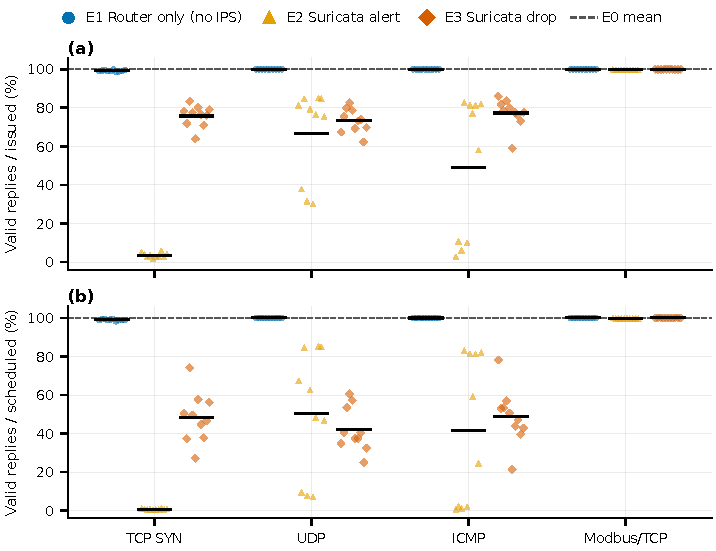
\includegraphics[width=0.88\textwidth]{r1_availability.pdf}
\caption{Availability of the SCADA client during the 60~s attack: (a) valid replies divided by requests issued; (b) valid replies divided by requests scheduled (10~Hz $\times$ 60~s). Each marker is one run, the black bar is the mean, and the dashed line is the baseline E0.}\label{fig:avail}
\end{figure}

Figure~\ref{fig:series} shows the same quantity per second. The service falls when the attack starts and recovers when it ends, except in E3, which stays at about 92\,\% in the 10~s after the attack (Section~\ref{sec:fp}). The Modbus flood does not affect the replies during the attack, but the PLC stops answering when the attack ends (Section~\ref{sec:modbus}).

\begin{figure}[H]
\centering
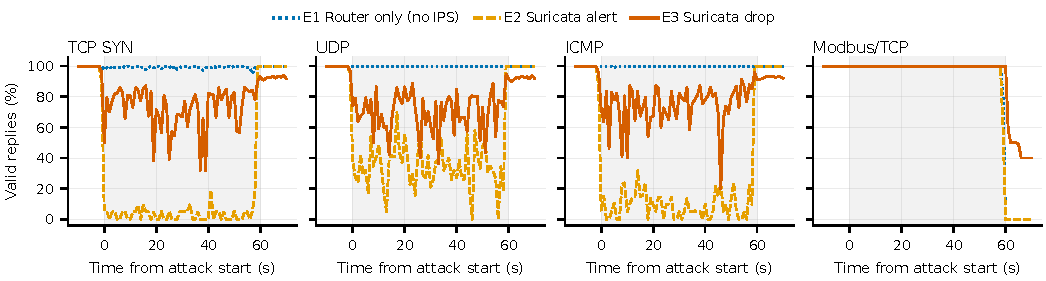
\includegraphics[width=0.92\textwidth]{r3_availability_timeseries.pdf}
\caption{Valid replies per second, averaged over the 10 runs of each combination. The shaded band is the attack window.}\label{fig:series}
\end{figure}

\subsection{Attack Traffic Removed and Resource Use}
The column Removed of Table~\ref{tab:results} gives the share of attack packets that do not reach the PLC network, measured on the mirror ports. In E3 the rules remove 99.7--100\,\% of the SYN, UDP, and ICMP floods. In E2 the rules only alert, so no packet is dropped by a rule (Suricata reported zero blocked packets), and the 54--69\,\% that disappears is due to the overflow of the \texttt{NFQUEUE}: the IPS cannot process the flood. In E1 only 0--2\,\% disappears; there is no IPS in that condition, so this difference is attributed to the packets that the capture tool discards. The packet counts are consistent across sources: for every run of E2 and E3, the packets that enter the queues (nftables counters, both directions) equal the packets dropped by the queue plus the verdicts of Suricata, with a ratio of 1.000 (0.998--1.006 in the Modbus runs of E3).

The CPU time of the virtual machines during the attack (hypervisor accounting, relative to the number of virtual CPUs) shows where the load goes. Without the IPS (E1), the PLC machine is close to saturation (82--103\,\% of its CPU) during the three volumetric floods and the Modbus flood. In E3 the PLC machine is nearly idle (about 1\,\%) because the attack does not reach it, while under the three volumetric floods the IPS machine uses all of its CPU time. The values can exceed 100\,\% because the CPU time of the hypervisor includes the emulation and I/O threads of each virtual machine. In other words, the inline IPS moves the bottleneck from the PLC to the IPS: it protects the PLC but its capacity limits the legitimate traffic that is forwarded.

\subsection{Statistical Comparison}
Table~\ref{tab:tests} gives the effect sizes and the significance of the comparisons for $A_{sch}$. Without the IPS (E1), the service is better than with the IPS (E2 and E3) in the three volumetric floods ($\delta=+1.00$, every run of E1 above every run of E2 and E3). Between E2 and E3, drop mode is better only for the SYN flood; for UDP and ICMP the difference is not significant, so the data do not show that dropping the packets by rule improves the replies over alerting them, because in both conditions the queue is the bottleneck. In the Modbus flood, E2 and E3 differ by a practically negligible amount (99.7\,\% against 100\,\%).

\begin{table}[H]
\caption{Cliff's $\delta$ for the first condition of each pair, replies/scheduled. Significance after Holm's correction: ns, not significant; $*$, $p<0.05$; $**$, $p<0.01$; $***$, $p<0.001$. Last row: $p$ values of Fisher's exact test for the PLC crashes.}\label{tab:tests}
\centering\footnotesize
\begin{tabular}{lccc}
\toprule
Attack & E1 vs E2 & E1 vs E3 & E2 vs E3\\
\midrule
TCP SYN & +1.00 (**) & +1.00 (**) & -1.00 (**)\\
UDP & +1.00 (***) & +1.00 (***) & +0.28 (ns)\\
ICMP & +1.00 (**) & +1.00 (**) & +0.00 (ns)\\
Modbus & +1.00 (***) & +0.00 (ns) & -1.00 (***)\\
\midrule
PLC down (Modbus), $p$ & 1.000 & 0.087 & 0.087\\
\bottomrule
\end{tabular}

\end{table}

\subsection{Modbus/TCP Flood and PLC Crash}\label{sec:modbus}
The Modbus flood sends valid requests at a low packet rate, so it does not degrade the replies during the attack in any condition (99.7--100\,\%). However, the OpenPLC runtime stopped when the attack ended in all runs of E1 and E2 (10 of 10) and in 6 of 10 runs of E3. In E3 the rule cuts the flow of the attacker, which sends only 46 packets per second on average, but the difference in crashes with E1 is not significant (Fisher, $p=0.087$). The Modbus flood therefore shows that the rate-based rules are not enough to protect the PLC runtime in this testbed.

\subsection{Detection and Rule Behavior}\label{sec:fp}
The rules produced alerts in all 80 runs of E2 and E3. For the SYN and ICMP floods in E3, the number of alerts is almost the number of packets processed by Suricata (99.8\,\%). For UDP, in contrast, the number of alerts is nearly constant, about 65\,500 per run, whatever the number of packets: in a calibration run with full alert logging (not part of the 130 runs), each alert corresponded to a different UDP source port, that is, one alert per flow and not one per packet. A per-packet detection rate is therefore reported only for SYN and ICMP, and the detection of UDP is reported per run and per flow.

The same calibration, repeated in four runs in drop mode with full logging, showed that the Modbus rule dropped 133--162 packets of the legitimate SCADA client per run, at the end of the 30~s attack and during the cool-down, when the client reconnects. This is a false positive of a rate-based rule, and it is consistent with the service not returning to 100\,\% right after the attack in E3 (Fig.~\ref{fig:series}). It does not explain the loss of replies during the attack, because the SCADA packets were not dropped by the rule during most of the attack. These false positives were not quantified in the 130 runs, in which the log only stored counters.

\subsection{Threats to Validity}
The measurements come from one physical host with virtual machines and a virtual switch, so absolute values (RTT, capacity of the IPS) are specific to this hardware and do not transfer to a physical PLC or industrial switch, which were not evaluated. The CPU time is measured in a virtual machine, and the capture tool discarded up to 13.8\,\% of the packets in some runs of E1. Six runs (five of E3 with ICMP and one of E1 with ICMP) started with the host colder than the others because of a defect in the temperature check of the scripts, which was corrected; their measurements are complete, and the sample does not allow attributing the lower E3 availability observed in them to the cold start. The Modbus rule was not recalibrated, and Snort was not evaluated.
